\documentclass[a4paper]{report}
% Shared preamble for the English probability and statistics documents.
% Based on the original course preamble. Compile with pdfLaTeX.
\usepackage[top=1.5cm,bottom=2cm,left=2cm,right=2cm]{geometry}
\usepackage[T1]{fontenc}
\usepackage{lmodern}
\usepackage[utf8]{inputenc}
\usepackage[english]{babel}

\usepackage{amsmath}
\usepackage{amssymb}
\usepackage{amsthm}
\usepackage{mathrsfs}
\usepackage{mathtools}
\usepackage{etoolbox}
\usepackage{tikz}
\usetikzlibrary{shapes.multipart,arrows.meta}
\usepackage{xcolor}
\usepackage{enumerate}
\usepackage[shortlabels]{enumitem}
\usepackage{hyperref}
\usepackage{version}
\usepackage{bbold}
\usepackage{fontawesome5}
\usepackage{fancyhdr}
\lfoot{}
\usepackage{natbib}
\usepackage{graphicx}
\usepackage{pdfpages}
\usepackage{authblk}
    
\usepackage{blindtext}
\usepackage{multicol}
\usepackage{collcell}
\usepackage{wrapfig}
\usepackage{blkarray}
\usepackage{cancel}
\usepackage{appendix}
\usepackage{float}
\makeatletter
\input{tex/assets/slashbox.sty}
\makeatother
\hypersetup{unicode,colorlinks,citecolor=red,filecolor=black,
  linkcolor=red,urlcolor=cyan}
\setlength{\columnsep}{1cm}
\pagenumbering{gobble}

\def\numtext#1{%
  \ifcase#1\or one\or two\or three\or four\or five\or six\or seven\or eight\or nine\or ten\or
  eleven\or twelve\or thirteen\or fourteen\or fifteen\or sixteen\or seventeen\or eighteen\or nineteen\or twenty\or Lots\fi}

\newcommand{\Byte}[1]{%
  \def\nodecontents{}%
  \foreach[count=\l] \k in {#1} {\xappto{\nodecontents}{\noexpand\nodepart{\numtext{\l}}\k}}%
  \node[rectangle split,rectangle split parts=8,rectangle split horizontal,draw] at (2,2){\nodecontents};}

\newcommand{\D}{{\mathrm{d}}}
\newcommand{\cE}{{\mathcal{E}}}
\newcommand{\cG}{{\mathcal{G}}}
\newcommand{\cX}{{\mathcal{X}}}
\newcommand{\cY}{{\mathcal{Y}}}
\newcommand{\cB}{{\mathcal{B}}}
\newcommand{\cF}{{\mathcal{F}}}
\newcommand{\cO}{{\mathcal{O}}}
\newcommand{\cS}{{\mathcal{S}}}
\newcommand{\cT}{{\mathcal{T}}}
\newcommand{\given}{\, \big| \,}
\newcommand{\cL}{{\mathscr{L}}}
\newcommand{\cD}{{\mathcal{D}}}
\newcommand{\cA}{{\mathscr{A}}}
\newcommand{\cP}{{\mathscr{P}}}
\newcommand{\cR}{{\mathscr{R}}}
\newcommand{\A}{{\mathcal A}}
\newcommand{\one}{\mathbb{1}}
\newcommand{\mathbbm}[1]{\mathbb{#1}}

\providecommand{\C}{}
\renewcommand{\C}{\mathbb C}
\newcommand{\R}{\mathbb R}
\newcommand{\Q}{\mathbb Q}
\newcommand{\N}{\mathbb N}
\newcommand{\T}{\mathbb T}
\newcommand{\F}{\mathbb F}
\renewcommand{\P}{\mathbb P}
\newcommand{\Z}{\mathbb Z}
\newcommand{\E}{\mathbb {E}}
\newcommand{\Pbb}[1]{\P\left( #1\right)}
\newcommand{\Ebb}[1]{\E\left[ #1\right]}

\newcommand{\lb}{\left (}
\newcommand{\rb}{\right )}
\newcommand{\lbb}{\left [}
\newcommand{\rbb}{\right ]}
\newcommand{\labs}{\left |}
\newcommand{\rabs}{\right |}
\newcommand{\lbrb}[1]{\lb #1 \rb}
\newcommand{\lbbrbb}[1]{\lbb#1\rbb}
\newcommand{\labsrabs}[1]{\labs#1\rabs}
\newcommand{\lbbrb}[1]{\lbb#1\rb}
\newcommand{\lbrbb}[1]{\lb#1\rbb}
\newcommand{\langlerangle}[1]{\langle#1\rangle}
\newcommand{\lbcurly}{\{}
\newcommand{\rbcurly}{\}}
\newcommand{\curly}[1]{\lbcurly#1\rbcurly}
\newcommand{\abs}{\labsrabs}
\newcommand{\ind}[1]{1_{#1}}
\newcommand{\indep}{\perp \!\!\! \perp}
\renewcommand{\d}{\, \mathrm{d}}

\newtheorem{theorem}{Theorem}
\newtheorem{problemCnt}{Lemma}
\theoremstyle{definition}
\newtheorem{problem}[problemCnt]{Problem}
\newtheorem{problembook}[problemCnt]{\faBook \,  Problem}
\newtheorem{problempencil}[problemCnt]{\faPencil* \,  Problem}
\newtheorem{problemstar}[problemCnt]{\faStar\,  Problem}
\newtheorem{problemstarpencil}[problemCnt]{\faStar \, \faPencil* \,   Problem}
\newtheorem{probleminteresting}[problemCnt]{\faSmile[regular] \,   Problem}
\newtheorem{solution}{Solution}

\newcommand{\fwcell}[1]{\makebox[\arraystretch\normalbaselineskip]{$#1$}}
\newenvironment{enumeratei}{\begin{enumerate}[(i)]}{\end{enumerate}}
\newenvironment{enumeratea}{\begin{enumerate}[(a)]}{\end{enumerate}}
\newenvironment{enumeraten}{\begin{enumerate}[\upshape 1.]}{\end{enumerate}}

% Compatibility helpers needed by a few files in the combined archive.
\AtBeginDocument{\noindent{\footnotesize English translation prepared with ChatGPT (OpenAI, GPT-6), 26 October 2026, for translation of the Bulgarian text into English and LaTeX formatting.
The Bulgarian originals remain the reference; translation may contain errors.}\par\smallskip}
\newcommand{\MissingGraphic}[1]{%
  \begin{center}\fbox{\parbox{0.82\linewidth}{\centering Missing source image: \texttt{#1}}}\end{center}}



\begin{document}
\noindent Computer Science, Year 3, Stream 2, 13 May 2023 \hfill Test 1
\hrulefill
\begin{it}The exact grading formula depends on the results. As an approximation, use 2 + the number of points. Time allowed: 3 hours. Good luck! Throughout, work on $(\Omega,\mathcal F,\P)$.\end{it}
\begin{problem}
A player in ``Gold Rush''\footnote{\url{https://bit.ly/3nRl2pG}, \url{https://bit.ly/3Bc0bjO}.} drops a ball into the top triangle of the pyramid of luck. At each level it falls into either lower triangle with equal probability.
\[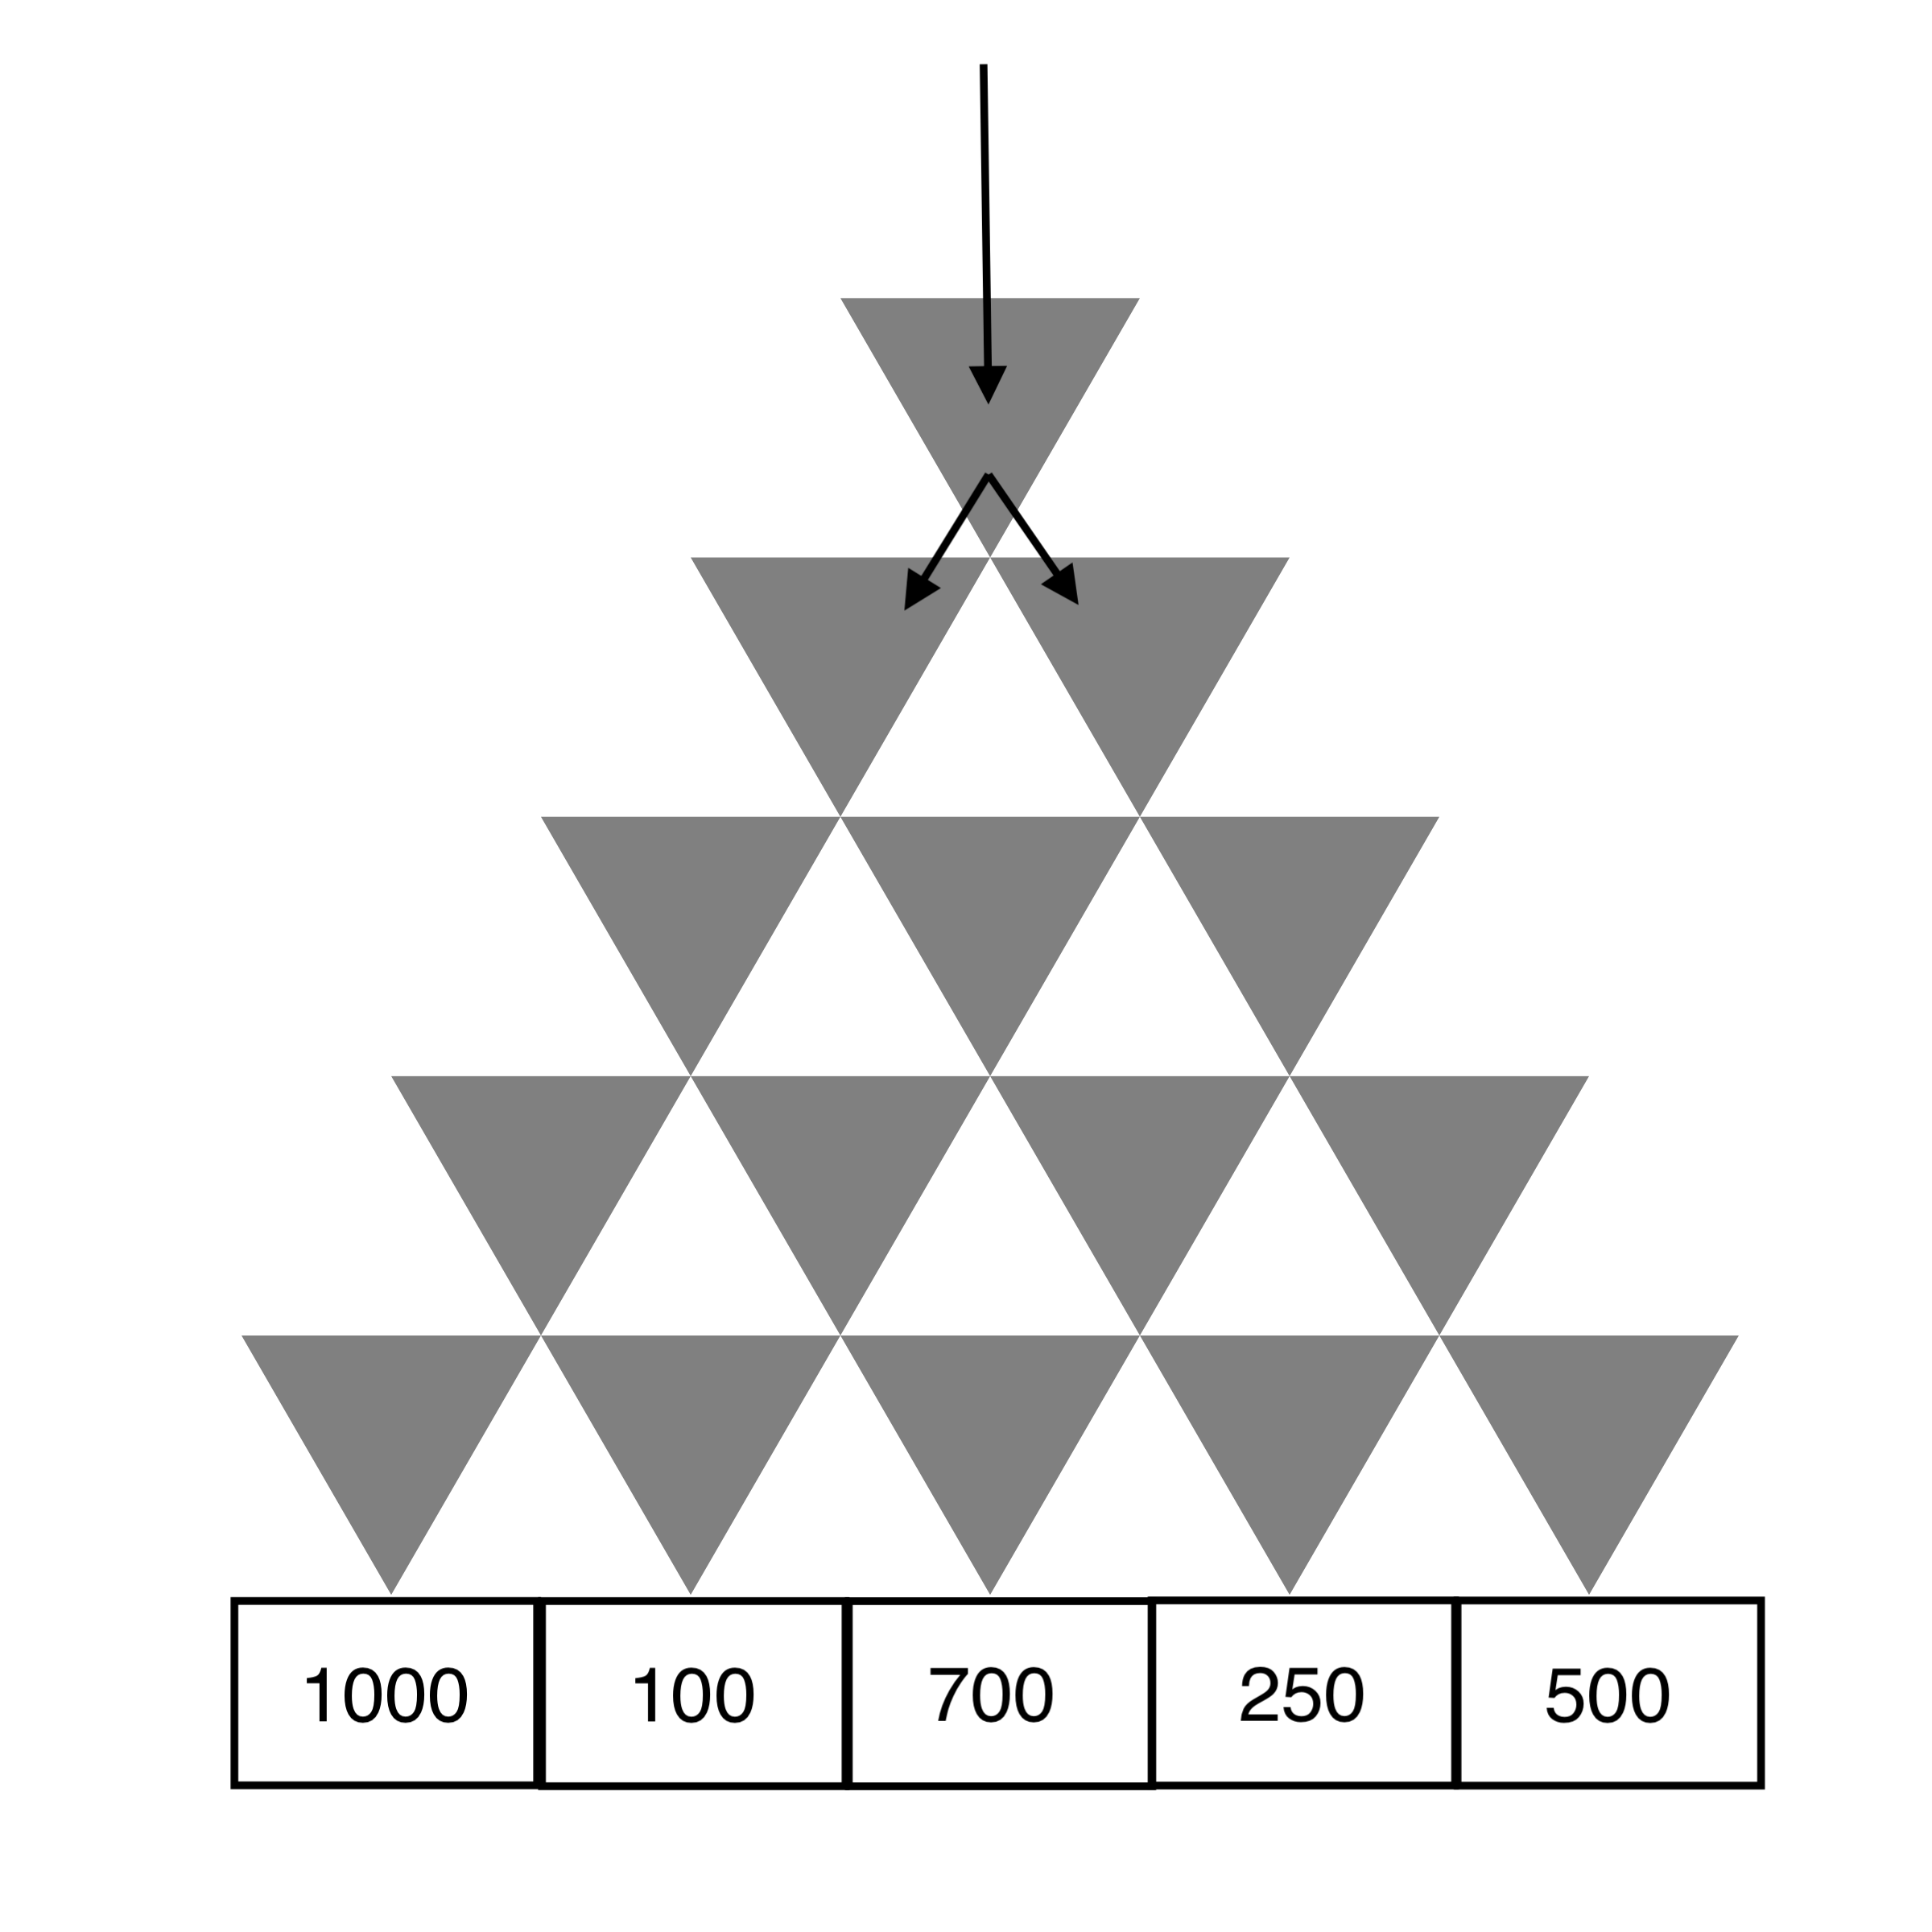
\includegraphics[width=0.4\textwidth]{tex/assets/prob-stat/triangles.png}\]
\begin{enumerate}
\item (0.5 points) Find the distribution and expected winnings from one drop.
\item (0.5 points) If you may continue until a ball lands in the 1000 BGN slot, how many balls will you drop on average? What are your expected winnings?
\item (0.5 points) The host offers to randomly permute the prizes. Would you accept or keep the initial arrangement? How would you arrange the prizes if allowed?
\end{enumerate}
You suspect the ball does not move left and right equally often. Let $p$ be the probability of moving left.
\begin{enumerate}[start=4]
\item (0.25 points) Three dropped balls all land in the 100 BGN slot. Which $p$ makes this most likely?
\item (0.5 points) The show has two pyramids, with $p=1/2$ and $p=1/3$, equally likely to be in use. Two drops both finish in the middle (700 BGN). What is the posterior probability that the $p=1/3$ machine was chosen?
\end{enumerate}
\end{problem}
\begin{problem} (1 point)
Consider $\mathrm{Ber}(p)$, $\mathrm{Bin}(n,p)$, $\mathrm{Ge}(p)$ and $\mathrm{Poi}(\lambda)$. For each law, let $X_1,X_2$ be iid. Does $X_1X_2$, or $X_1+X_2$, have the same distributional type as $X_1$, possibly with different parameters? Justify all four cases. If not always, give an example where this situation does occur.
\end{problem}
\begin{problem}
Let $X_1,X_2,X_3$ be iid with mean $\mu$ and variance $\sigma^2$. An observer wishes to estimate $\E f(X_1,X_2,X_3)$ from one realization $(x_1,x_2,x_3)$. One method uses $f(x_1,x_2,x_3)$. Another artificially adds the permutations $(x_2,x_1,x_3)$, $(x_3,x_2,x_1)$ and $(x_1,x_3,x_2)$, averaging all four results. Compare the accuracy by calculating the expectations and variances when:
\begin{enumerate}
\item (0.1 points) $f=X_1+X_2+X_3$;
\item (0.2 points) $f=X_1+X_2-X_3$;
\item (0.7 points) $f=X_1X_2-X_3$.
\end{enumerate}
\emph{Example: for $(3,8,1)$ in part 3, the first estimate is $3\cdot8-1=23$. Adding $(8,3,1)$, $(1,8,3)$ and $(3,1,8)$ gives the second estimate $[(3\cdot8-1)+(8\cdot3-1)+(1\cdot8-3)+(3\cdot1-8)]/4=11.5$.}
\end{problem}
\end{document}
